%%
%% 研究報告用スイッチ
%% [techrep]
%%
%% 欧文表記無しのスイッチ(etitle,eabstractは任意)
%% [noauthor]
%%

%\documentclass[submit,techrep]{ipsj}
\documentclass[submit,techrep,noauthor]{ipsj}

\usepackage{latexsym}
\usepackage{booktabs}
\usepackage{url}
\usepackage{nidanfloat}
\usepackage{afterpage}
\usepackage{setspace}
\usepackage{multirow}
\usepackage{here}
\usepackage{amsmath,amssymb}
\usepackage{bm}
%\usepackage{graphicx}
\usepackage[dvipdfmx]{graphicx}
\usepackage{subcaption}
\captionsetup{compatibility=false}
\usepackage{verbatim}
\usepackage{wrapfig}
\usepackage{ascmac}
%\bibliographystyle{unsrt}
\usepackage{algorithm}
\usepackage{algorithmic}

\def\Underline{\setbox0\hbox\bgroup\let\\\endUnderline}
\def\endUnderline{\vphantom{y}\egroup\smash{\underline{\box0}}\\}
\def\|{\verb|}
%

%\setcounter{巻数}{59}%vol59=2018
%\setcounter{号数}{10}
%\setcounter{page}{1}


\begin{document}


\title{画像付きフェイクニュースとジョークニュースの\\
検出・分類に向けた機械学習モデルの検討}

\affiliate{UEC}{電気通信大学\\
UEC, Chofu, Tokyo 182--8585, Japan}

\author{柳 裕太}{Yuta Yanagi}{UEC}[yanagi.yuta@ohsuga.lab.uec.ac.jp]
\author{田原 康之}{Yasuyuki Tahara}{UEC}[ohsuga@uec.ac.jp]
\author{大須賀 昭彦}{Akihiko Ohsuga}{UEC}[tahara@uec.ac.jp]
\author{清 雄一}{Yuichi Sei}{UEC}[seiuny@uec.ac.jp]

\begin{abstract}
    %背景
    SNSの発展によりあらゆる情報入手が容易になった反面,人を欺くために故意に作成された虚偽の情報であるフェイクニュースが社会問題になっている.
    特に画像と併せて発信されたものは,テキストのみならず画像と併せた分析アプローチが有効である.
    虚偽の情報としては,もう1つジョークニュースというものもある.
    これは人を欺くためではなく,社会風刺や皮肉のために作られた情報という特徴がある.
    しばしばこの2カテゴリが混同され,ジョークニュースが批判に晒されることがあることも問題となっている.

    %既存課題
    既にテキスト・画像をニューラルネットワークの一種であるCNNによって分析して真偽を判定する自動判別モデルが提案されている.
    実際に真実・フェイクとのカテゴリ分類において優秀な成績を収めているものの,
    ジョークとしての嘘情報と人を欺くための嘘情報が区別されていない.


    %提案
    本研究では,正しい情報・ジョークニュース・フェイクニュースの3カテゴリを分類することで,より画像つきフェイクニュースの検出精度を向上させることを目指した.


    %実験結果
    実際にSNSから収集した画像つきのデータセットを対象にカテゴリ分類を行った結果,3カテゴリでもマクロF値が約0.93と良好な結果を示した.
\end{abstract}
%

%
%\begin{jkeyword}
%情報処理学会論文誌ジャーナル,\LaTeX,スタイルファイル,べからず集
%\end{jkeyword}
%
%\begin{eabstract}
%This document is a guide to prepare a draft for submitting to IPSJ
%Journal, and the final camera-ready manuscript of a paper to appear in
%IPSJ Journal, using {\LaTeX} and special style files.  Since this
%document itself is produced with the style files, it will help you to
%refer its source file which is distributed with the style files.
%\end{eabstract}
%
%\begin{ekeyword}
%IPSJ Journal, \LaTeX, style files, ``Dos and Dont's'' list
%\end{ekeyword}

\maketitle

% 背景[フェイクニュースの自動判別の必要性+ジョークニュースを区別する必要性]+想定環境の説明(導入との被りに注意)
\section{序論}
\label{ch:introduction}
%
% フェイクニュース
昨今のSNSの普及により,誰もが情報を発信・収集できるようになった.
特に最近ではテキストのみならず,画像や動画と併せて情報の発信が可能である.
一般論として,テキスト単体と比べて画像や動画と併せて発信されたマルチメディア情報の方が多くの注目を得やすい.
逆にこれを利用して,故意に情報を捏造して発信することによって人々を誤った方向へ扇動するフェイクニュースも存在する.
フェイクニュースが広まると、大規模なマイナスの影響が出る可能性があり、
場合によっては重要な公共の出来事に影響を及ぼしたり、操作したりすることさえある.
例えば2016年の米国大統領選では,2名の候補者を支持させるためのフェイクニュースが多く拡散され,
とりわけFacebook上では3700万回以上共有された\cite{10.1257/jep.31.2.211}.

% ジョークニュース
虚偽の情報ながら,扇動ではなく皮肉や風刺を込めたジョークニュースも存在する.
有名な発信メディアとしては,英語ではthe Onion,日本語では虚構新聞が該当する.
あくまで扇動ではなく笑いを提供するためのものであり,
多くの場合それは批判の的にはなりにくかった.
しかしながら,ジョークニュースはフェイクニュースと同じく限りなく真実を模した形式をとるため,
昨今では同じくSNS上で拡散されやすく,同時に批判に晒されることもある.

% 想定環境
当研究では,扇動のために故意に情報を捏造して発信された情報をフェイクニュース,
事実を発信した情報を正しいニュース,
そして風刺や皮肉を込めて発信された情報をジョークニュースとして定義する.

% フェイクニュースのテキストによる分類
フェイクニュースに限らず,風評やwebページの信憑性を評価するモデルの構築の研究は数多く行われており,
特に機械学習による分類が非常に盛んに行われている.
なかでもGranikらの研究\cite{Granik8100379}やGildaの研究\cite{Gilda8305411},そして松尾の研究\cite{松尾省吾2018master}により,
単語埋め込みとナイーブベイズ分類器やSVM,決定木といった教師あり学習を組み合わせることによって,
フェイクニュースや流言を分類するタスクで優秀な分類成果を挙げることが報告された.
ほかにもWuらの研究\cite{Wu:2018:TFF:3159652.3159677}によると,SNS上で拡散された情報に対して,
``誰が・どのような経緯で拡散したか''という情報から信憑性を判断するモデルも提案された. 
Rubinらの研究\cite{W16-0802}によれば,正しいニュース・ジョークニュースの分類にも機械学習によるアプローチが有効であることが示されていた.
正しいニュース・フェイクニュース・ジョークニュースの3カテゴリ分類においても研究が行われている.
特にHorneとSibelの研究\cite{DBLP:journals/corr/HorneA17}によると,フェイクニュースは正しいニュースよりジョークニュースに近い性質をもち,
真実に近い形式をとるほど高い説得力をもつことが示されていた.

% マルチメディアでフェイクニュース分類
上記の機械学習を使った研究では,いずれもテキストのみの情報を対象としていた.
別の対象として,テキスト・画像を併せた情報を分類する機械学習モデルの検討も数多く行われている.
大まかな形としては,まずテキスト・画像を何らかの方法でベクトル化する.
その後2種のベクトルを結合し,真偽判定を行うモデルに渡す形をとっている.
例えばJinらの研究\cite{Jin:2017:MFR:3123266.3123454}では,テキストではLSTM,画像ではVGG19を使用してベクトル化しており,
それに加えてAttentionとソーシャルコンテキスト(ハッシュタグ,URL等)により更に高精度な分類を行うモデルが提案されていた.
またWangらの研究\cite{Wang:2018:EEA:3219819.3219903}では,EANNというモデルが提案されている.
これは画像のベクトル化においては同じくVGG19を使用しているが,テキストではテキストCNNを使用していた.

上記のEANNモデルのような画像・テキスト双方を扱うモデルでは,実際に真実・フェイクとのカテゴリ分類において画像単独・テキスト単独の分類に比べて優秀な成績を収めていた\cite{Wang:2018:EEA:3219819.3219903}.\@
しかしながら,あくまで``真実なのかそうでないのか''という2カテゴリで分類しているため,
``他者を欺くための情報なのか,皮肉・風刺を込めた情報なのか''という観点での分析がなされていない.

% 本研究
本研究では,画像つきで発信された情報に対して,正しい情報か・フェイクニュースか・ジョークニュースかを判断するモデルを構築する.
このモデルを使い,従来から画像・テキスト複合のデータセットに対して3カテゴリでも優秀な分類が行えることを示すことを目指す.
それにより,SNSユーザの情報収集を支援するエージェントの開発につなげることが可能となる.

% 実験
上記の提案する情報分類システムを検証するために,
事前に用意されたデータセットを用いて10 分割交差検定によって分析を行った.
また上記システムの分類性能を評価するために,
画像・テキスト単独で分類を行った結果と比較することで,
提案システムが目標に適していることを示すことを目指した.
その結果テキスト単独でのマクロF値が約0.30,画像単独でのマクロF値が約0.47であったのに比べ,
提案モデルのマクロF値は約0.93という数値を出し,提案モデルの有効性が示された.

\section{関連研究}
\subsection{画像・文章の分析}
画像分類のは近年目まぐるしい発展を遂げた.
特に画像の被写体から分類するタスクにおいては,
VGG19のように16-19層の畳み込み層(CNN)を取り入れたモデルが非常に高い分類成果を挙げることが報告
\cite{DBLP:journals/corr/SimonyanZ14a}された.
また,VGG19を含めた多くのモデルでは,事前学習済みモデルが配布されているため,自分で転移学習を行うことも容易である.
文章に関しても,画像と同じく並列実行が可能なCNNをテキスト用にアレンジしたテキストCNNも提案
\cite{DBLP:journals/corr/Kim14f}され,広く使われている.

画像と文章を組み合わせた研究も数多くなされてきた.
例えば,画像をCNNで分析してLSTMによってキャプションを生成する研究\cite{7298935}によって,
より精度の高いキャプション生成ができたことが報告された.
他にも画像に対して文章で視覚質問(画像に写ったものを問う)
に応答することを目的としたVQA\cite{7410636}というモデルも提案された.

\subsection{フェイクニュース対策}
現在,フェイクニュースを判断する手法の1つに有識者によって事実関係を確認するファクトチェックがある.
例えばPolitifact.comではTruth-o-meterという独自指標によって,
政治的主張に対して疑わしさを7段階で評価\cite{holan_2018}している.

フェイクニュース自体への対策が発展していく中で,
フェイクニュースを``真実か嘘か''という基準から判断すること自体に疑義を唱える取り組みも存在する.
現在,Mike Tamir氏によって立ち上げられたFakerFactというwebアプリケーションがある\cite{tamir}.
このwebサイトではWaltという独自のAIを搭載しており,
文章を``真実か嘘か''は判断せず,文章の論調を分類していた.

このようにフェイクニュースを判断するにあたって,
近年では``真実か嘘か''という観点にとらわれない多くのアプローチや分類が行われていることがわかる.

\section{研究目的}
\label{ch:purpose}
%
今回対象とするカテゴリの投稿例を今回扱ったデータセットから抜粋したものが以下の図\ref{fig:examples}である.

\begin{figure*}[ht]
    \centering
    \begin{subfigure}[b]{0.4\textwidth}
        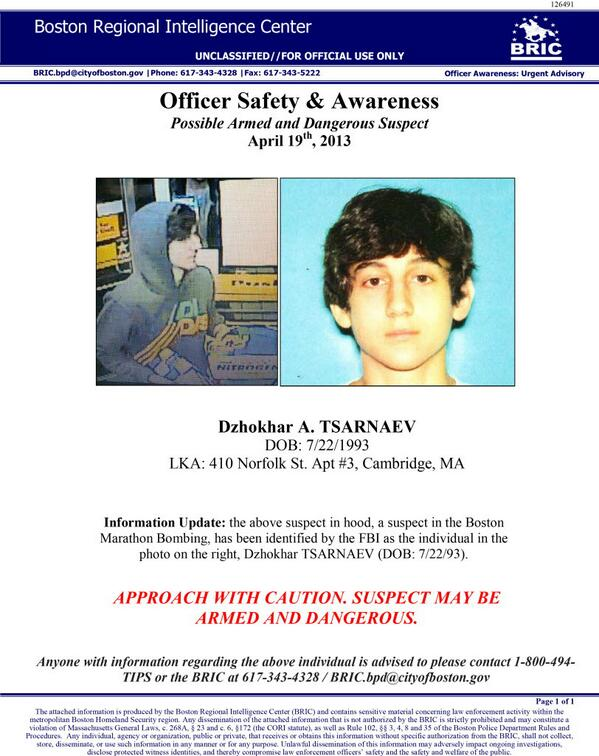
\includegraphics[height=6.5cm]{images/real_example_boston.jpg}
        \caption{Boston RIC released this flier showing at large suspect Dzhokhar Tsarnaev. He may be armed \& dangerous}
        \label{fig:real}
    \end{subfigure}
    \hfill % separation between the subfigures
    \begin{subfigure}[b]{0.57\textwidth}
        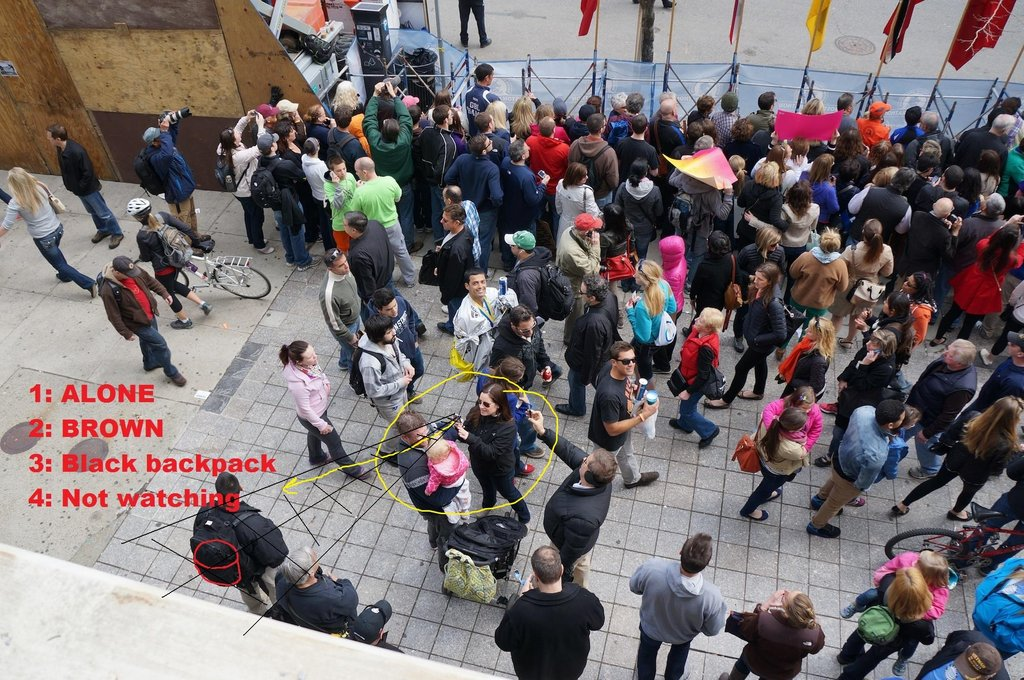
\includegraphics[height=6.5cm]{images/humor_example_boston.jpg}
        \caption{The detail of these photos used to identify the Boston Marathon bombing suspect is bananas…}
        \label{fig:humor}
    \end{subfigure}
    \bigskip 
    \centering
    \begin{subfigure}[b]{\textwidth}
        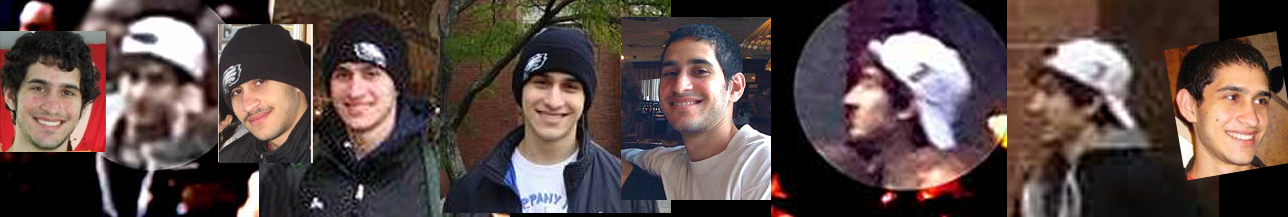
\includegraphics[width=\textwidth]{images/fake_example_boston.jpg}
        \caption{Reddit is on to something... Boston Bomber \#2 sure looks like missing student Sunil Tripathi. }
        \label{fig:fake}
    \end{subfigure}
    \caption{当研究で扱う3カテゴリの投稿例: (a)正しいニュース,(b)ジョークニュース,(c)フェイクニュース}
    \label{fig:examples}
\end{figure*}

いずれも2013年に発生したボストンマラソン爆弾テロ事件に関してTwitter上で投稿されたものであった.
図\ref{fig:real}は実際にボストン市傘下が作成した被疑者の情報をChicago Sun-TimesがTwitterに投稿したもの,
図\ref{fig:humor}はテロ後にRedditや4chanにて有志が実行犯の調査が行われた件に対して
``bananas''と茶化すような言葉を投げかけているもの,
図\ref{fig:fake}は実際に上記掲示板上で実行犯の調査が行われた結果,
全くの別人を槍玉に挙げているものである.

実際に,ボストンマラソン後ではインターネット上で盛んに犯人探しが行われた結果,
事件前に行方不明になっていたスニル・トリパティ(Sunil Tripathi)さんが犯人として扱われ,
更にその後一般報道メディアもトリパティさんの家族に取材が行われるなど,
フェイクニュースが実害として現実になった\cite{gray_2013}.
これを受け,Redditでは実際に犯人探しの過熱で無関係の個人とその家族に迷惑をかけたとして謝罪した\cite{laird_2013}.

%
当研究では,上記対象を正確に3カテゴリへ分類するモデルを構築することを目標としている.
具体的には,入力として画像と文章を持ち,それに対してどのカテゴリが該当するかを出力するモデルとなる.

当研究を更に発展させると,SNS上でユーザや運営側を支援するエージェント開発に繋げることができる.
%
%
\section{提案手法}
%
\subsection{モデル概観}
この章では,提案モデルがもつ複合特徴量抽出器とニュース分類器について紹介する.
その後にこの2要素を統合して転移学習が可能な表現を学習する方法について説明する.
% 最後に,詳細なアルゴリズムフローを付加する. 
今回提案したモデルは,以下の図\ref{fig:model}の通りである.

提案モデルの目的は,画像と文章で発信された情報に対して,
正しいニュースか・フェイクニュースか・ジョークニュースかを分類するために,
必要な特徴表現を学習することであった.
提案モデルは複合特徴量抽出器とニュース分類器の大きく2部分に分けることができた.
まず複合特徴量抽出器は,今回扱う情報が文章と画像を含むため,
各メディアに対して特徴化する抽出器があった.
その後それぞれの特徴を1つに連結し,複合特徴を形成した.
複合特徴はニュース分類器に送られ,最終的には3カテゴリのどれに該当するかが判断された.
% 
\begin{figure}[tb]
    \centering
    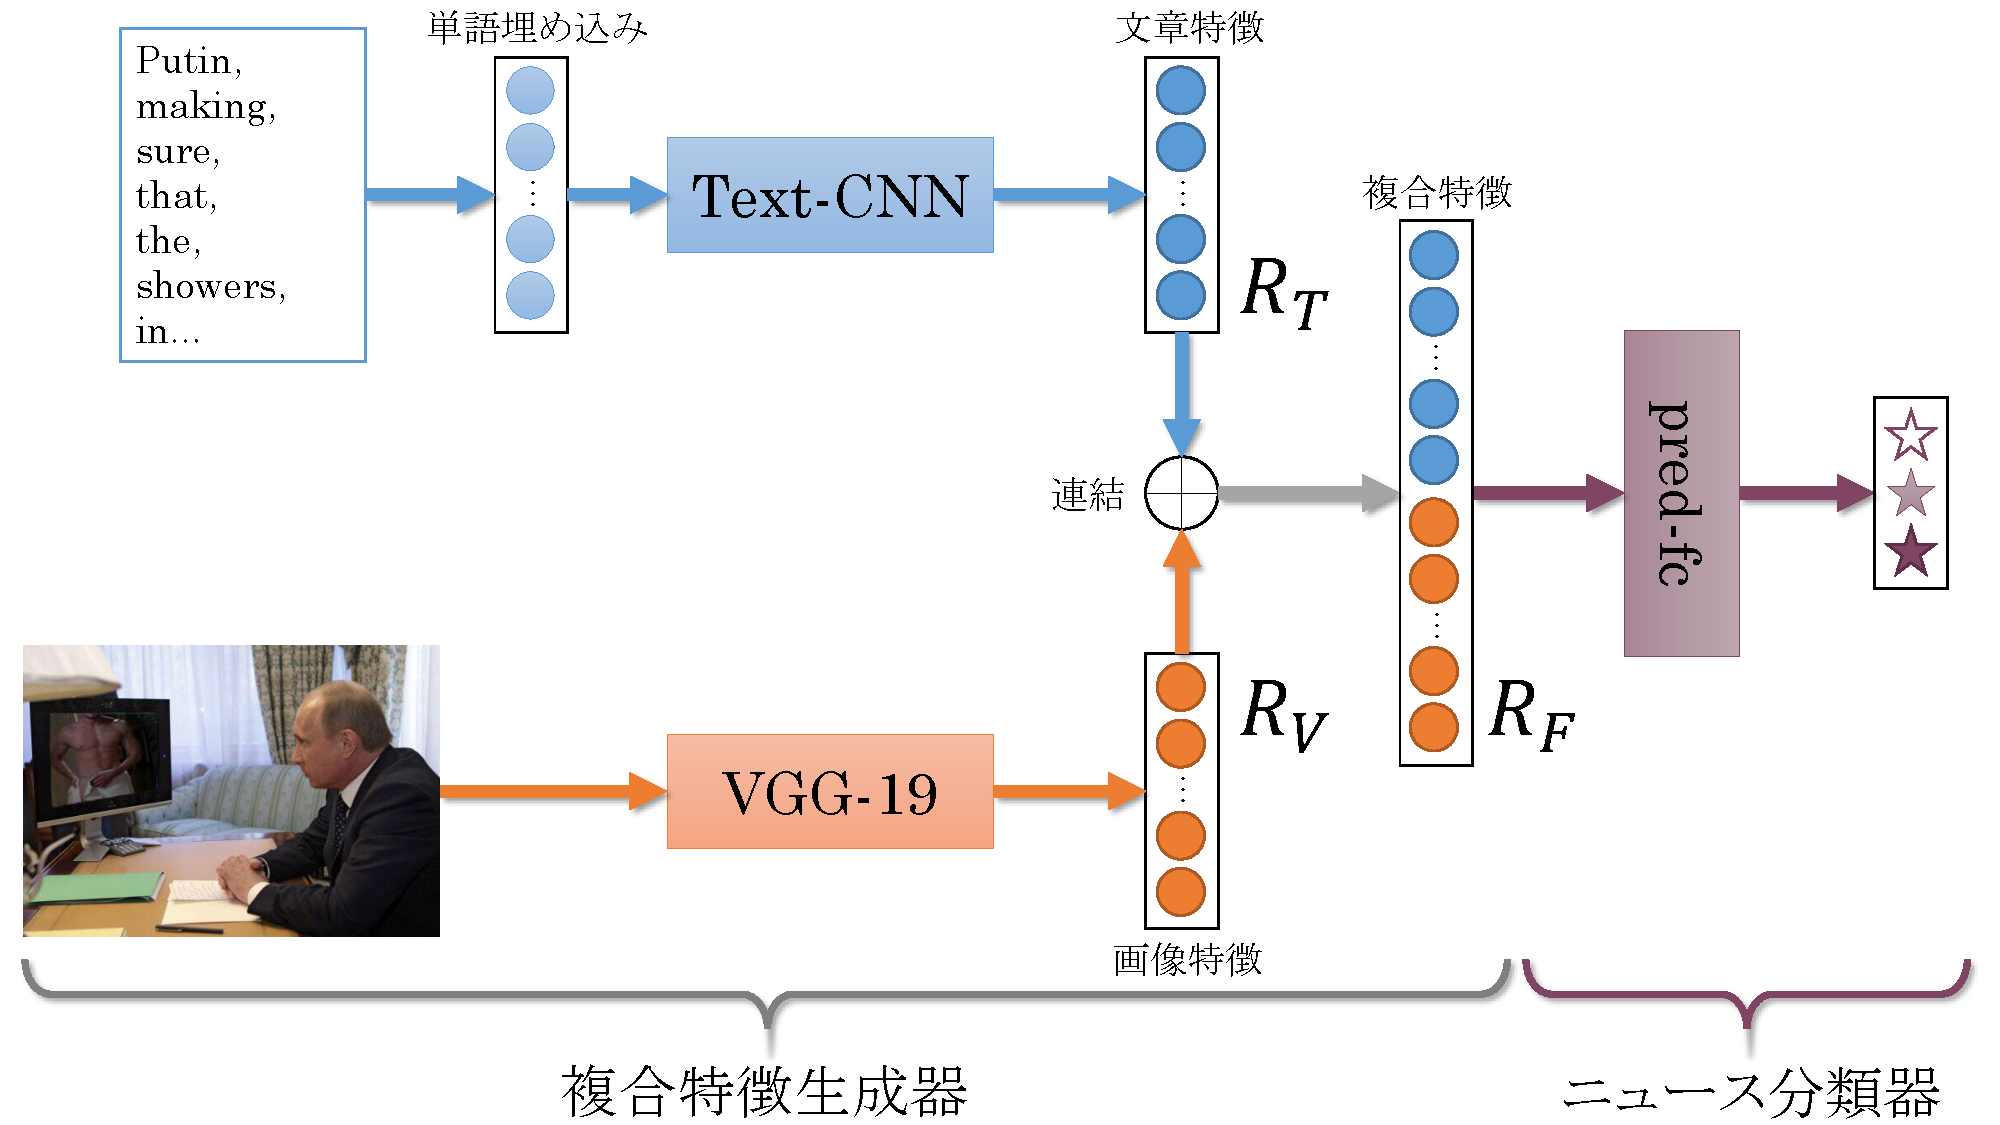
\includegraphics[width=0.8\linewidth]{images/methodology.pdf}
    \caption{提案モデル図.青: 文章特徴量抽出器,橙: 画像特徴抽出器,紫: ニュース分類器.}
    \label{fig:model}
\end{figure}
%
\subsection{複合特徴抽出器}
%
\subsubsection{文章特徴} \label{subsec:text}
文章特徴は,入力に英語の投稿をスペース毎に分割した英単語の連続リストをもった.
まずは単語を単語埋め込みでベクトル化した.
その後単語の羅列から分類に有効な情報を得るために,文章特徴を抽出する核としてCNN
(convolutional neural networks: 畳み込みニューラルネットワーク)を採用した.
CNNはコンピュータビジョンやテキスト分類などの多くの分野で効果的であることが示されていた
\cite{collobert2011natural,KalchbrennerACL2014}.
図\ref{fig:model}の通り,提案手法ではCNNの発展形であるテキストCNN(Text-CNN)\cite{DBLP:journals/corr/Kim14f}を採用した.
テキストCNNの構造は図\ref{fig:text-cnn}の通りである.
複数のウィンドウで畳み込むことで,様々な角度から特徴を抽出することを実現した.
\begin{figure}[H]
    \centering
    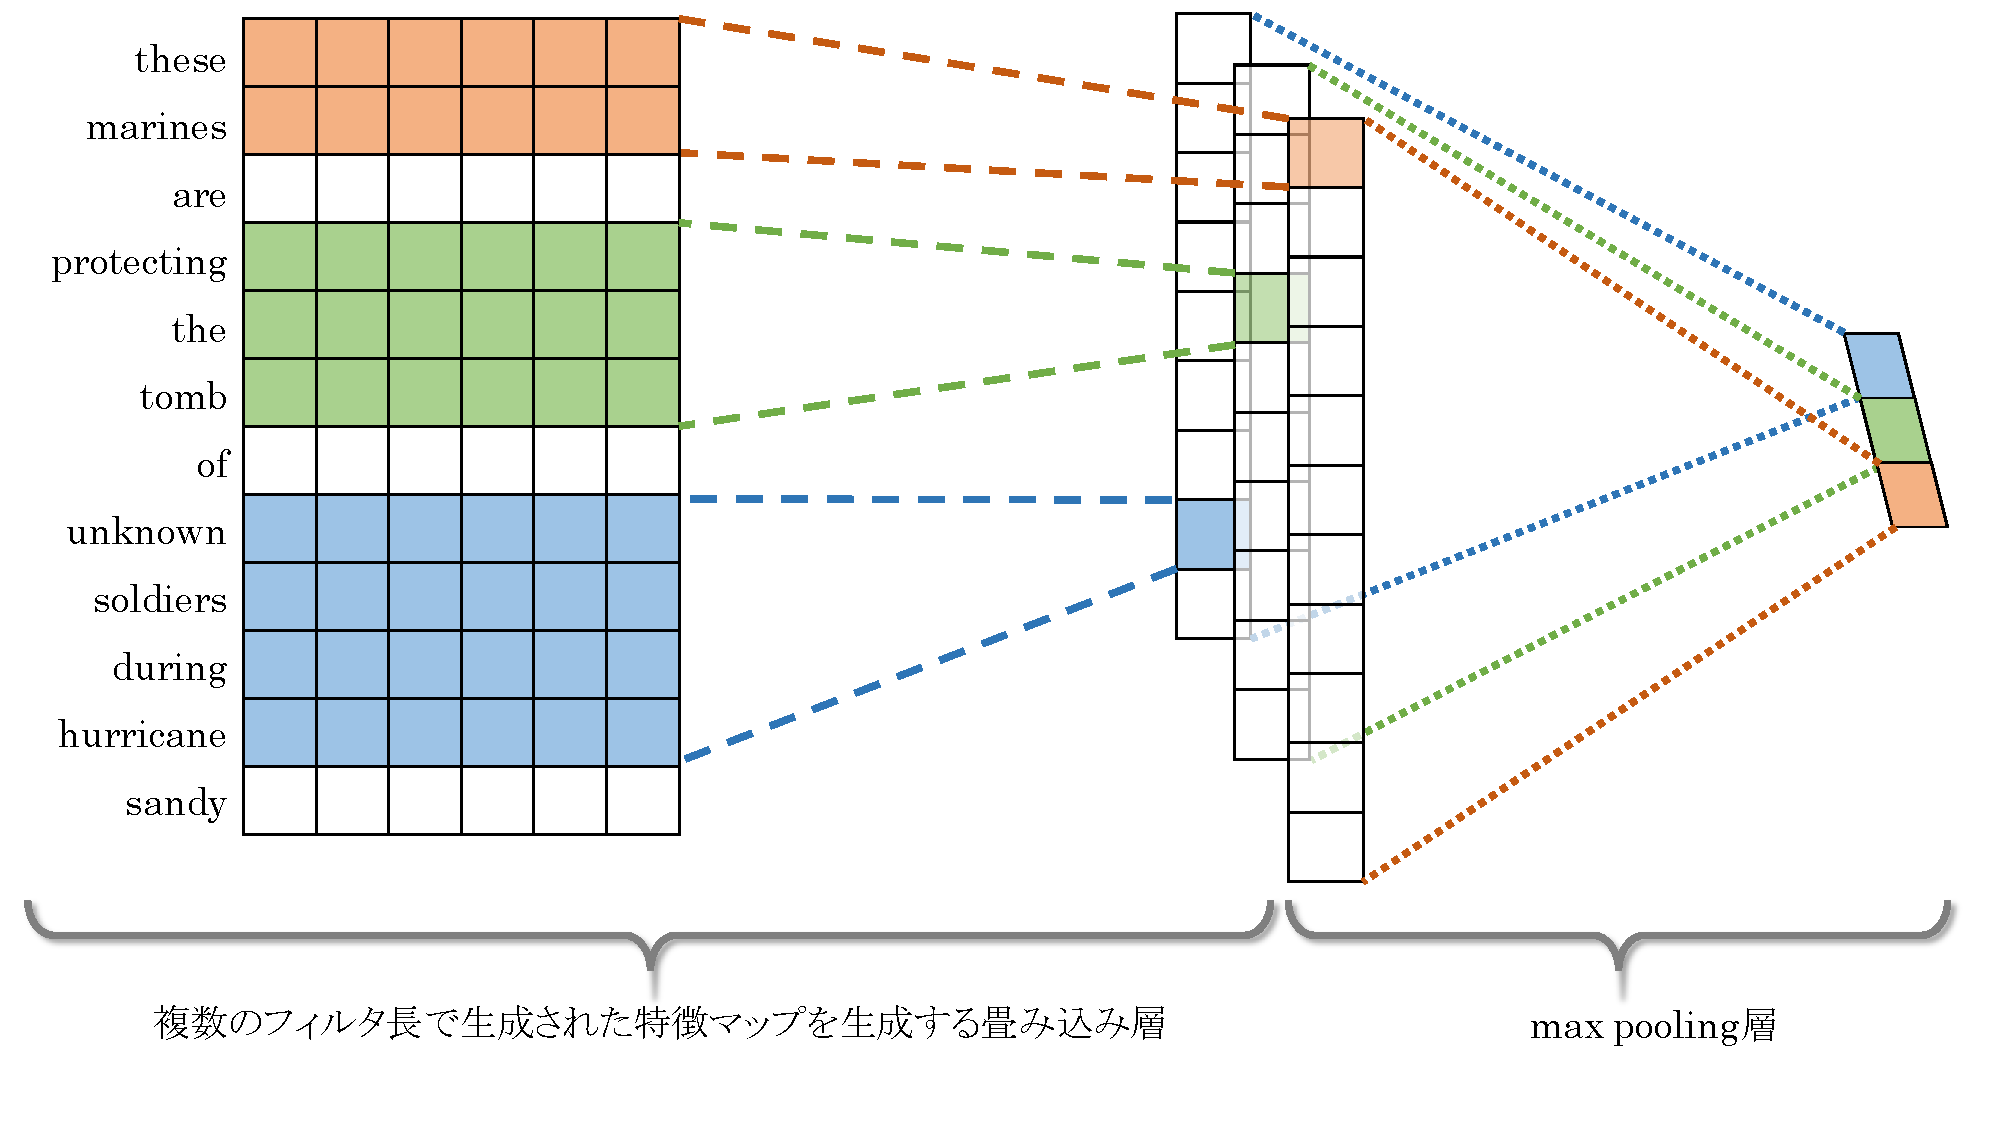
\includegraphics[width=\linewidth]{images/text-cnn.pdf}
    \caption{テキストCNNの図.Wangらの研究\cite{Wang:2018:EEA:3219819.3219903}を参考に作成.}
    \label{fig:text-cnn}
\end{figure}

具体的な手法では,EANNが採用したテキストCNNと同じ流れを汲み\cite{Wang:2018:EEA:3219819.3219903},
最終の全結合層の隠れ層に独自にdropoutを採用した形をとった.
今回使用した文章特徴抽出器の理論式を以下に引用する.

投稿の$i$番目の単語を$k$次元の単語埋め込みに変換する際に抽出された単語埋め込みベクトルを$T_i \in \mathbb{R}^k$とする.
このとき,$n$単語から抽出された投稿は以下の式\ref{eq:concat_emb}で表現ができる.
\begin{equation}
    \label{eq:concat_emb}
    T_{1:n} = T_1 \oplus T_2 \oplus \ldots \oplus T_n,
\end{equation}
$\oplus$はベクトルを連結(concatenation)することを意味する記号である.
ここで単語埋め込み化された投稿は,畳み込み層へ送られる.
畳み込み層では$h$単語分のウィンドウサイズがある.
これは単語埋め込み化された投稿から連続して取り出す単語埋め込みベクトルの数を意味する.
$i$番目を基準に$h$単語分取り出された場合,フィルタ時の処理は以下の式\ref{eq:filter}の通りである.
\begin{equation}
    \label{eq:filter}
    t_i = \sigma(W_c \cdot T_{i:i+h-1}).
\end{equation}
この$\sigma(\cdot)$は活性化関数の1つであるReLU(ランプ関数)を表し,$W_c$はフィルタの重みを意味する.
式\ref{eq:filter}が投稿内で適用されると,式\ref{eq:feature}の通り1つの発言に対し1つの特徴ベクトルが得られる.
\begin{equation}
    \label{eq:feature}
    t = [t_1, t_2, \ldots, t_{n-h+1}].
\end{equation}
この$t$ベクトルに対して最も重要な特徴を得るために,ベクトル内で最大値の要素のみを取り出すmax-poolingが行われる.

これで1つのウィンドウサイズから1つの特徴が得られるが,
多くの粒度の特徴を得るために当手法では複数のウィンドウサイズから複数の値を取得している.
特定のウィンドウサイズに着目すると,$n_h$分異なるフィルタが存在することになる.
もし使用可能なウィンドウサイズが$c$存在する場合,全体で$c \cdot n_h$だけフィルタが存在することとなる.
投稿から各ウィンドウサイズでmax-poolingまでされた文章特徴は$R_{T_c} \in \mathbb{R}^{c \cdot n_h}$と表現できる.

max-poolingを終えた文章特徴は全結合層に渡され,
最終的に式\ref{eq:image-fc}によって
画像特徴抽出器が出力する特徴ベクトルの次元($p$とする)に合わせたテキスト特徴$R_T \in \mathbb{R}^p$となる.
\begin{equation}
    \label{eq:image-fc}
    R_T = \sigma(W_{tf} \cdot R_{t_c}),
\end{equation}
ここで$W_{tf}$は全結合層における重みを意味する.なお,この全結合層では隠れ層にdropoutを当研究では採用した.
dropoutはHintonらによって提案された手法\cite{JMLR:v15:srivastava14a}で,
学習時に指定された確率で無作為に$W_{tf}$内の要素を無効化(0に)してモデルの自由度を制限することで,
モデルが訓練データセットに特化しすぎて汎用性が失われる過学習に繋がりにくくなる利点が報告されたものであった.
%
\subsubsection{画像特徴}
画像から効率的に特徴を抽出するために,当研究では事前学習済みのVGG19\cite{DBLP:journals/corr/SimonyanZ14a}を起用した.
VGG19は畳み込み16層と全結合層3層から形成され,最終的には1000次元の特徴ベクトルが出力される.
当研究では最終の全結合層のみ改変し,文章特徴のベクトル次元数と同じ数の次元をもつベクトルを出力するようにした.
また改変した最終全結合層以外は,過学習を防ぐために事前学習の状態を維持することにした.

第\ref{subsec:text}節で記したように,最終的な特徴ベクトルの次元数は$p$とする.
VGG19では畳み込み16層で$7 \times 7 \times 512$の行列となり,
その後2層の全結合層によって$1 \times 1 \times 4096$に整形され,
最終第三全結合層(fc19)によって$1 \times 1 \times 1000$の画像特徴ベクトルを出力する.
Wangらの研究\cite{Wang:2018:EEA:3219819.3219903}ではVGGのfc19の出力を$p$に整形していたが,
当研究では直接fc19を改変して$1 \times 1 \times p$の画像特徴ベクトルを出力するようにした.
この改変したfc19によって算出される画像特徴$R_V \in \mathbb{R}^p$は以下の式\ref{eq:fc19}の通りである.
\begin{equation}
    \label{eq:fc19}
    R_V = \sigma(W_{vf} \cdot R_{V_{\rm VGGfc18}}),
\end{equation}
$R_{V_{\rm VGGfc18}}$はVGG19の第18層である全結合層が出力した$1 \times 1 \times 4096$ベクトルである.

こうして文章特徴・画像特徴が抽出され,最終的には2つの特徴ベクトルを1つに連結したものが複合特徴である.
理論式で表記すると,文章特徴$R_T$と画像特徴$R_V$が1つに結合されるため,
複合特徴$R_F$は以下の式\ref{eq:concat_feature}によって表現できる.
\begin{equation}
    \label{eq:concat_feature}
    R_F = R_T \oplus R_V \in \mathbb{R}^{2p}.
\end{equation}
以降においては,複合特徴抽出器全体を表現するときは$G_f(M; \theta_f)$と表現することにする.
$M$は複合特徴抽出器へ入力される投稿,$\theta_f$は学習対象となるパラメータを意味する.
%
\subsection{ニュース分類器}
%
複合特徴はニュース分類器(図\ref{fig:model}内`pred-fc'が該当)にて正しいニュース・フェイクニュース・ジョークニュースとして分類された.
具体的には隠れ層を含む全結合層とsoftmaxから形成され,最終的な分類が行われた.
この部分の理論式は以下の通りである.

入力となる複合特徴は$R_F$であるとき,ニュース分類器は$G_f(\cdot; \theta_d)$と表現することにする.
ここで$\theta_d$はニュース分類器内で学習対象となるパラメータを示す.
投稿全体に対して$i$番目の投稿を$m_i$とするとき,
$m_i$がフェイクニュースもしくはジョークニュースである確率は以下の式によって算出される.
\begin{equation}
    \label{eq:news_classify}
    P_\theta(m_i) = G_d(G_f(M; \theta_f); \theta_d).
\end{equation}
モデルの目的は自動で正確に正しいニュース・フェイクニュース・ジョークニュースを分類することである.
そのため正解ラベルとして$Y_d$を使用して,以下の式によってクロスエントロピー誤差を損失として算出する.
\begin{multline}
    \label{eq:cross_entropy}
    L_d(\theta_f, \theta_d) =\\
    -\mathbb{E}{(m,y)~(M, Y_d)}[y\log P_\theta(m) + (1-y)\log (1-P_\theta(m))].
\end{multline}

最後に,当研究がベースとしたWangらの研究では確率的勾配降下法(SGD: Stochastic Gradient Descent)
によってパラメータを更新していたが,
当研究では2015年にDiederik P. Kingmaらが提唱したAdamという手法\cite{DBLP:journals/corr/KingmaB14}
を用いてパラメータを更新することにした.
%


%
\section{評価実験}
\label{ch:experiment}
%
\subsection{データセット}
今回の実験での訓練データセットでは,
Boididouらの研究\cite{boididou2015verifying}によって提案されたTwitter投稿データセットを使用した.
こちらもTwitter上でフェイクニュースを検出するために作られたデータセットであるが,
付加されたラベルとしてReal, Fake, そしてHumorがあり,
ジョークニュースを含めた3カテゴリ分類に適したものとなっているため,当研究で採用した.
データセットでは訓練用と検証用として2部に分かれていたが,
当研究では訓練用とされた部分の画像とテキストを対象に10分割交差検定することにした.

% 
\subsection{比較対象手法}
今回,画像つき文章投稿を3カテゴリに分類する提案手法の有効性を調べるために2種類の比較対象手法を用意した.
1つは文章のみで投稿を分類する手法(以降,Textと表記),もう1つは画像のみで投稿を分類する手法(以降,Imageと表記)であった.
いずれも上記提案モデルから文章・画像特徴抽出器を除外したモデルを使用した.
またTextは入力データを提案モデルが使用したデータセットから画像を削除したものを使用した.
Imageは全投稿で使用された画像を対象とし,同じ画像に対して複数の文章投稿があった場合は1件として数えることにした.
% 
\subsection{実験条件}
%
\subsubsection{Text}
モデルに入力する前に,単語埋め込みへの変換の事前処理として,スムーズに単語埋め込みに変換できるようにするために,
投稿からハッシュタグ(\#)のような記号を除去し,全ての大文字を小文字に変換してスペースで分割した.
投稿から分割された各単語を単語埋め込みに変換する際は,
Google Newsデータセットから事前学習済みのword2vecモデル\cite{google_2013}を使用した.
このモデルでは,各単語を300次元のベクトルに変換するものであった.
ここでwod2vecモデルに該当しない単語が出現した場合,\texttt{<unknown>}としてseed値固定ランダムベクトルを生成することにした.
また,投稿の全単語中50\%以上が\texttt{<unknown>}の場合,実態に則さない学習を避けるために学習対象から外すことにした.
その後テキストCNNに送られ,1つの文章に対して1つの300次元の特徴ベクトルが抽出され,ニュース分類器に渡す形となった.
なお,ウィンドウサイズは2-5までの4種類を用意し,全結合層の隠れ層は1つ用意し,ユニット数は300とした.
隠れ層では50\%のユニットが無視されるDropoutを導入した.
ニュース分類器内でも隠れ層は1つ用意し,ユニット数は300,上記と同じ条件のDropoutも導入した.
%
\subsubsection{Image}
モデルの複雑化を避けるため,1つの投稿に複数枚画像が付加されていた場合は最初の1枚のみをモデルに入力させることにした.
画像は事前学習済みVGG19モデルに入力し,1つの画像に対して1つの300次元のベクトルが抽出され,ニュース分類器に渡す形となった.
本来のVGG19は最終層にて1000次元のベクトルが出力されるが,最終層のみ改変して300次元のベクトルが出力されるようにした.
また前記の通り過学習を避けるために最終層を除き事前学習済みの状態を維持させることにした.
ニュース分類器の条件は上記Textと同一であった.
%
\subsubsection{提案手法}
提案手法では,TextとImageを統合した形をとったため,画像・文章の部分は上記と同様の条件をとった.
画像・文章の特徴を結合するため,ニュース分類器に渡されるのは600次元のベクトルであった.
それにあわせ,隠れ層のユニット数も600とした.
%
\subsection{使用データ統計}
上記の条件を踏まえ,提案手法・Text・Imageが扱う3カテゴリの投稿件数は以下の表\ref{table:posts}の通りである.
Textが使用するデータは提案手法が扱うデータから画像を削除したものであるため,提案手法と全く同じ件数になった.
Imageは,同じ画像に対して複数の投稿があったため,他2手法と比べて非常に少なくなっている.

\begin{table}[ht]
    \caption{提案手法と比較対象手法が扱うカテゴリ毎の投稿数}
    \label{table:posts}
    \centering
    \begin{tabular}{clll}
        \hline
        手法 & Real & Fake & Humor \\
        \hline \hline
        Text & 3021 & 4233 & 1509 \\
        Image & 172 & 157 & 82 \\
        提案手法 & 3021 & 4233 & 1509 \\
        \hline
    \end{tabular}
\end{table}

\subsection{評価指標}
評価指標では,Precision(精度), Recall(再現率), F値(左2値の調和平均)を使用することにした.
算出する方法上各カテゴリ毎に上記指標があるが,今回使用するデータセットでは極端にカテゴリが偏っていないので,
各カテゴリの指標を先に算出してから3カテゴリの平均をとるマクロ平均を評価に使うことにした.

\subsection{実験結果}
3モデルに対して10分割交差検定を行った結果が以下の表\ref{table:result}の通りである.
% 
\begin{table}[ht]
    \caption{各モデルの分類成果(マクロ平均)}
    \label{table:result}
    \centering
    \begin{tabular}{clll}
        \hline
        手法 & Precision & Recall & F値 \\
        \hline \hline
        Text & 0.3649 & 0.3677 & 0.3016 \\
        Image & 0.4942 & 0.5055 & 0.4667 \\
        提案手法 & 0.9268 & 0.9362 & 0.9286 \\
        \hline
    \end{tabular}
\end{table}

この結果を見ると,提案手法が他2手法と比べて非常に高い分類成果を挙げたことが読み取れた.
また,比較対象手法内で比べると画像単体の方が分類成果が良好である点もみられた.

\section{評価}

\subsection{考察}
今回の評価実験では,提案手法が3指標全てにおいて比較対象手法より優れた分類成績を収めた.
これにより,SNS上で画像つきの投稿を対象にした場合,正しいニュース・フェイクニュースの分類タスクのみならず,
ジョークニュースも含めた分類においても従来のマルチメディアモデルのアプローチが有効であることが示唆されたと考えられる.

また比較対象手法に限って結果を観察すると,文章単体より画像単体の分類の方が優秀な分類成績であった.
これは自然言語より画像の方が分類タスクにおいて研究が進んでいることや,
SNS上の投稿であった故に単語埋め込みに変換する際に\texttt{<unknown>}に変換されやすい傾向にあったことや,
文章の場合英語以外の投稿に対応できないものの,画像においては英語圏以外の投稿であっても十分言語の違いに影響されにくかったことなど,
いくつかの原因が推察される.

\subsection{課題}
今回分類するにあたり,大きな課題となったのが文章投稿の単語埋め込みへの変換であった.
使用したデータがSNS上から収集されたものであったため,
事前学習済みword2vecモデルが対応できない短縮語や造語(ハッシュタグ含)といったユーザ生成コンテンツに対応することが難しかった.

また,当モデルに限らずフェイクニュース検出というタスクにおいて,Wangらの研究\cite{Wang:2018:EEA:3219819.3219903}で問題点が指摘されていた.
訓練データセットが扱ったイベントや出来事の特殊性の影響で,別のイベントや出来事に対して正常な判断ができなくなる点であった.

さらに,このモデルは英語のみを対象としたものであった点も挙げられた.
データセット内一部では他国の言語が含まれていたため,単語埋め込みに変換する際に大幅に\texttt{<unknown>}に変換される傾向もあった.
%
%
\section{おわりに}
%
\subsection{本論文のまとめ}
本研究では,SNS上で画像と文章を併せて発信された情報に対して,正しいニュース・フェイクニュース・ジョークニュースを判断するモデルを提案した.
実際に3カテゴリ分類を行った結果,文章・画像単体から分類した場合に比べて,全ての評価指標において非常に優秀な分類成績を挙げた.
これによりSNS上における画像つき投稿に対して,ジョークニュースを含めた3カテゴリ分類も有効であることが示された.
%
\subsection{今後の展望}
このモデルの発展形として,いくつかの方法が考えられる.

例えば文章特徴生成器に対して,テキストCNNではなくVosoughiらの研究\cite{Vosoughi:2016:TLT:2911451.2914762}によってSNS投稿を分析するために提案された,
文字単位でベクトル変換する方法を採用することなどが考えられる.

また,データセットが扱う出来事やイベントによる特殊性の対策として,
Wangらの研究\cite{Wang:2018:EEA:3219819.3219903}では敵対的生成ネットワーク(GAN)を模倣する形をとることが挙げられていた.
このイベントや出来事による特殊性を排するために,真偽分類に加えて扱われたイベントも分類することによって,
特徴化する際に特殊性を排し,フェイクニュースの普遍的な特徴を抽出するようなアプローチが行われていた.
実際にこれによって分類精度が改善した点が上記研究によって報告されていたため,当研究でも有効に働く可能性がある.

提案手法を日本語投稿に対応させることを考えた場合,
まずSNS上で日本語による画像つきの3カテゴリの投稿を収集する必要があると考えられる.
もしも既に日本語投稿による3カテゴリ分類済みのデータセットがあれば投稿を収集する必要はないが,
残念ながら国内に今回使用したデータセットに近い規模をもつものがないのが現状である.

% 

%謝辞
\section*{謝辞}
\addcontentsline{toc}{section}{謝辞}
本研究はJSPS科研費JP16K00419, JP16K12411, JP17H04705, JP18H03229,
JP18H03340, JP18K19835の助成を受けたものです.

%また,研究の機会と議論・研鑽の場を提供して頂き,ご指導頂いた国立情報学研究所/東京大学の本位田真一教授をはじめ活発な議論と貴重なご意見を頂いた研究グループの皆様,大須賀・田原研究室の皆様に感謝の意を表します.さらに,本研究を行う上で必要な楽天公開データの提供に協力してくださいました国立情報学研究所,楽天株式会社の関係者の皆様に感謝の意を表します.

%\section*{研究業績}
%\addcontentsline{toc}{section}{研究業績}

%\subsection*{国際会議}
%\begin{achievement}
%\item \underline{\textbf{Minato Sato}}, Ryohei Orihara, Sei Yuichi, Yasuyuki Tahara and Akihiko Ohsuga: Japanese Text Classification by Character-Level Deep ConvNets and Transfer Learning, The 9th International Coneference on Agents and Artificial Intelligence (ICAART2017), Feb 2017. (accepted as a Full Paper)
%\end{achievement}

%\subsection*{査読付き国内シンポジウム・ワークショップ}
%\begin{achievement}
%\item \underline{\textbf{佐藤挙斗}},折原良平,清雄一,田原康之,大須賀昭彦: 文字レベル深層学習による日本語テキストの分類と転移学習,合同エージェントワークショップ&シンポジウム2016 (JAWS2016),pp.199-206,2016年9月. (ショート発表) \textcolor{red}{{\bf 優秀発表賞}}
%\end{achievement}

%\subsection*{研究会}
%\begin{achievement}
%\item \underline{\textbf{佐藤挙斗}},折原良平,清雄一,田原康之,大須賀昭彦: 文字レベル深層学習の日本語データセットへの応用,第184回 情報処理学会 知能システム研究会 (SIG-ICS) ,2016年8月.
%\item \underline{\textbf{佐藤挙斗}},折原良平,清雄一,田原康之,大須賀昭彦: 文字レベル深層学習によるテキスト分類と転移学習,人工知能学会 第102回人工知能基本問題研究会(SIG-FPAI),2016年12月. 
%\end{achievement}

\begin{thebibliography}{10}

\bibitem{10.1257/jep.31.2.211}
Hunt Allcott and Matthew Gentzkow.
 Social media and fake news in the 2016 election.
 {\em Journal of Economic Perspectives}, 31(2):211--36, 5 2017.

\bibitem{Granik8100379}
M.~Granik and V.~Mesyura.
 Fake news detection using naive bayes classifier.
 In {\em 2017 IEEE First Ukraine Conference on Electrical and Computer
  Engineering (UKRCON)}, pages 900--903, 5 2017.

\bibitem{Gilda8305411}
S.~Gilda.
 Evaluating machine learning algorithms for fake news detection.
 In {\em 2017 IEEE 15th Student Conference on Research and Development
  (SCOReD)}, pages 110--115, 12 2017.

\bibitem{松尾省吾2018master}
松尾 省吾.
 機械学習を用いた流言の検出に関する研究.
 Master's thesis, 電気通信大学院, 2018.

\bibitem{Wu:2018:TFF:3159652.3159677}
Liang Wu and Huan Liu.
 Tracing fake-news footprints: Characterizing social media messages by
  how they propagate.
 In {\em Proceedings of the Eleventh ACM International Conference on
  Web Search and Data Mining}, WSDM '18, pages 637--645, New York, NY, USA,
  2018. ACM.

\bibitem{W16-0802}
Victoria Rubin, Niall Conroy, Yimin Chen, and Sarah Cornwell.
 Fake news or truth? using satirical cues to detect potentially
  misleading news.
 In {\em Proceedings of the Second Workshop on Computational
  Approaches to Deception Detection}, pages 7--17. Association for
  Computational Linguistics, 2016.

\bibitem{DBLP:journals/corr/HorneA17}
Benjamin~D. Horne and Sibel Adali.
 This just in: Fake news packs a lot in title, uses simpler,
  repetitive content in text body, more similar to satire than real news.
 {\em CoRR}, abs/1703.09398, 2017.

\bibitem{Jin:2017:MFR:3123266.3123454}
Zhiwei Jin, Juan Cao, Han Guo, Yongdong Zhang, and Jiebo Luo.
 Multimodal fusion with recurrent neural networks for rumor detection
  on microblogs.
 In {\em Proceedings of the 25th ACM International Conference on
  Multimedia}, MM '17, pages 795--816, New York, NY, USA, 2017. ACM.

\bibitem{Wang:2018:EEA:3219819.3219903}
Yaqing Wang, Fenglong Ma, Zhiwei Jin, Ye~Yuan, Guangxu Xun, Kishlay Jha, Lu~Su,
  and Jing Gao.
 Eann: Event adversarial neural networks for multi-modal fake news
  detection.
 In {\em Proceedings of the 24th ACM SIGKDD International Conference
  on Knowledge Discovery \&\#38; Data Mining}, KDD '18, pages 849--857, New
  York, NY, USA, 2018. ACM.

\bibitem{DBLP:journals/corr/SimonyanZ14a}
Karen Simonyan and Andrew Zisserman.
 Very deep convolutional networks for large-scale image recognition.
 {\em CoRR}, abs/1409.1556, 2014.

\bibitem{DBLP:journals/corr/Kim14f}
Yoon Kim.
 Convolutional neural networks for sentence classification.
 {\em CoRR}, abs/1408.5882, 2014.

\bibitem{7298935}
O.~Vinyals, A.~Toshev, S.~Bengio, and D.~Erhan.
 Show and tell: A neural image caption generator.
 In {\em 2015 IEEE Conference on Computer Vision and Pattern
  Recognition (CVPR)}, pages 3156--3164, 6 2015.

\bibitem{7410636}
S.~Antol, A.~Agrawal, J.~Lu, M.~Mitchell, D.~Batra, C.~L. Zitnick, and
  D.~Parikh.
 Vqa: Visual question answering.
 In {\em 2015 IEEE International Conference on Computer Vision
  (ICCV)}, pages 2425--2433, 12 2015.

\bibitem{holan_2018}
Angie~Drobnic Holan.
 The principles of the truth-o-meter: How we fact-check, 2 2018.

\bibitem{tamir}
Mike Tamir.
 About fakerfact.

\bibitem{harmanci_2012}
Reyhan Harmanci.
 11 viral photos that aren't hurricane sandy, 10 2012.

\bibitem{collobert2011natural}
Ronan Collobert, Jason Weston, L{\'e}on Bottou, Michael Karlen, Koray
  Kavukcuoglu, and Pavel Kuksa.
 Natural language processing (almost) from scratch.
 {\em Journal of Machine Learning Research}, 12(Aug):2493--2537, 2011.

\bibitem{KalchbrennerACL2014}
Nal Kalchbrenner, Edward Grefenstette, and Phil Blunsom.
 A convolutional neural network for modelling sentences.
 {\em Proceedings of the 52nd Annual Meeting of the Association for
  Computational Linguistics}, 6 2014.

\bibitem{JMLR:v15:srivastava14a}
Nitish Srivastava, Geoffrey Hinton, Alex Krizhevsky, Ilya Sutskever, and Ruslan
  Salakhutdinov.
 Dropout: A simple way to prevent neural networks from overfitting.
 {\em Journal of Machine Learning Research}, 15:1929--1958, 2014.

\bibitem{DBLP:journals/corr/KingmaB14}
Diederik~P. Kingma and Jimmy Ba.
 Adam: {A} method for stochastic optimization.
 {\em CoRR}, abs/1412.6980, 2014.

\bibitem{boididou2015verifying}
Christina Boididou, Katerina Andreadou, Symeon Papadopoulos, Duc-Tien
  Dang-Nguyen, Giulia Boato, Michael Riegler, Yiannis Kompatsiaris, et~al.
 Verifying multimedia use at mediaeval 2015.
 In {\em MediaEval}, 2015.

\bibitem{google_2013}
Tomas Mikolov and Ilya Sutskever.
 Google code archive - long-term storage for google code project
  hosting., 7 2013.

\bibitem{Vosoughi:2016:TLT:2911451.2914762}
Soroush Vosoughi, Prashanth Vijayaraghavan, and Deb Roy.
 Tweet2vec: Learning tweet embeddings using character-level cnn-lstm
  encoder-decoder.
 In {\em Proceedings of the 39th International ACM SIGIR Conference on
  Research and Development in Information Retrieval}, SIGIR '16, pages
  1041--1044, New York, NY, USA, 2016. ACM.

\end{thebibliography}

\end{document}
